\documentclass[10pt,c,ignorenonframetext]{beamer}
\renewcommand{\emph}[1]{\textcolor{blue}{\bf #1}}

%%*************************************%
\author[C. de Falco]{Carlo de Falco}
\institute[]{}
%**************************************%
\renewcommand{\emph}{\alert}

\usepackage[]{multimedia}
\usepackage[]{xmpmulti}
\usepackage[]{listings}
\usepackage[]{amsfonts}
\usepackage{t1enc}
\usepackage{subfigure}
\usepackage{times}

\lstset{language=C++,stringstyle=\color{green}, %
identifierstyle=\color{blue}\tt\bfseries, %
keywordstyle=\color{blue},commentstyle=\color{brown}\small\tt}

\newcommand{\comment}[1]{\center{\textcolor{blue}{\bf #1}}}
\newcommand{\of}[1]{\left( #1 \right)}
\newcommand{\ofv}[1]{\left[ #1 \right]}
\newcommand{\grad}{\vec{\nabla}}
\newcommand{\divg}[1]{\text{div} \left(#1 \right)}
\newcommand{\R}{\mathbb{R}}
\newcommand{\Po}{\mathbb{P}}
\newcommand{\Le}{\mathbb{L}}
\newcommand{\Pe}{\mathbb{P}e}
\newcommand{\Hd}{ H^{\text{div}}}
\newcommand{\norm}[1]{\left\| #1 \right\|}
\newcommand{\abs}[1]{\left| #1 \right|}
\newcommand{\dual}[1]{#1^{\prime}}
\newcommand{\vect}[1]{\mathbf{#1}}
\renewcommand{\vec}[1]{\mathbf{#1}}
\newcommand{\dz}[2]{#1^{\prime} \of{x}}
\newcommand{\dzm}[2]{#1^{\prime}} %{\frac{d #1}{d #2}}
\newcommand{\dztwo}[2]{#1^{\prime \prime} \of{x} }%{\frac{d^2 #1}{d #2^2}}
\newcommand{\pztwo}[2]{\frac{\partial^2 #1}{\partial #2^2}}
\newcommand{\bern}[2]{{\cal B}  \of{#2 #1 }}
\newcommand{\bernmod}[3]{{\cal B} \of{#2 #1 \ofv{#3} }}
\newcommand{\restr}[2]{{#1}_{#2}}
\newcommand{\restri}[2]{\left. #1\right|_{#2}}
\newcommand{\Ne}{N_{\text{ele}}}
\newcommand{\Nn}{N_{\text{nod}}}
\newcommand{\I}{\mathcal{I}}
\newcommand{\half}{\frac{1}{2}}
\newcommand{\harm}[2]{\exp \left[H_{#1}\left(#2\right)\right]}
\newcommand{\curl}[1]{\vec{curl\,}\of{#1}}
\newcommand{\Div}[1]{div\,\of{#1}}
\newcommand{\ep}{\psi}
\newcommand{\fp}{\phi}
\newcommand{\rb}[1]{\left( #1 \right)}

\graphicspath{{../figures/}}

%--------------------------------------%
\usetheme[]{pacs}

\AtBeginSubsection[\inserttocsection]
{
  \begin{frame}<beamer>{Outline}
    \tableofcontents[currentsection,currentsubsection]
  \end{frame}
}

\AtBeginSection[]
{
  \begin{frame}<beamer>{Outline}
    \tableofcontents[currentsection]
  \end{frame}
}
\title{PACS 2013-2014 Lab 01}
\date{11/10/2013}
\begin{document}
\begin{frame}
  \titlepage
\end{frame}

\section{Hello World!}

\begin{frame}
\begin{itemize}
\item Online resources
\begin{itemize}
\item Beep
\item GitHub
\end{itemize}
\item Contact
\begin{itemize}
\item Carlo de Falco: {\tt carlo.defalco@polimi.it}
\item Guido Iori: {\tt guidofr.iori@gmail.com}
\end{itemize}
\end{itemize}

\end{frame}

\begin{frame}[fragile]
\frametitle{Hello World! I}

The infamous ``Hello World!'' program:

\begin{lstlisting}
#include <iostream>

int main (void)
 {
   std::cout << "Hello World!" << std::endl;
   return 0;
 }
\end{lstlisting}

edit and save as {\tt helloworld.cpp}

\begin{lstlisting}[language=bash]
$ touch helloworld.cpp
$ emacs helloworld.cpp
\end{lstlisting}

\end{frame}

\begin{frame}[fragile]
\frametitle{Hello World! II}

Let's make it work:

\begin{lstlisting}[language=bash]
$ which g++
$ g++ --version
$ source /opt/src/setenvironment 
$ module avail
$ module load gcc/4.8.0
$ module list
$ which g++
$ g++ --version
\end{lstlisting}

now we are ready to build the executable

\begin{lstlisting}[language=bash]
$ g++ -c helloworld.cpp
$ g++ -o helloworld helloworld.o
\end{lstlisting}

and run it

\begin{lstlisting}[language=bash]
$ ./helloworld
\end{lstlisting}

Congratulations!!

\end{frame}

\begin{frame}
\frametitle{Excercise 1: IEEE double representation}
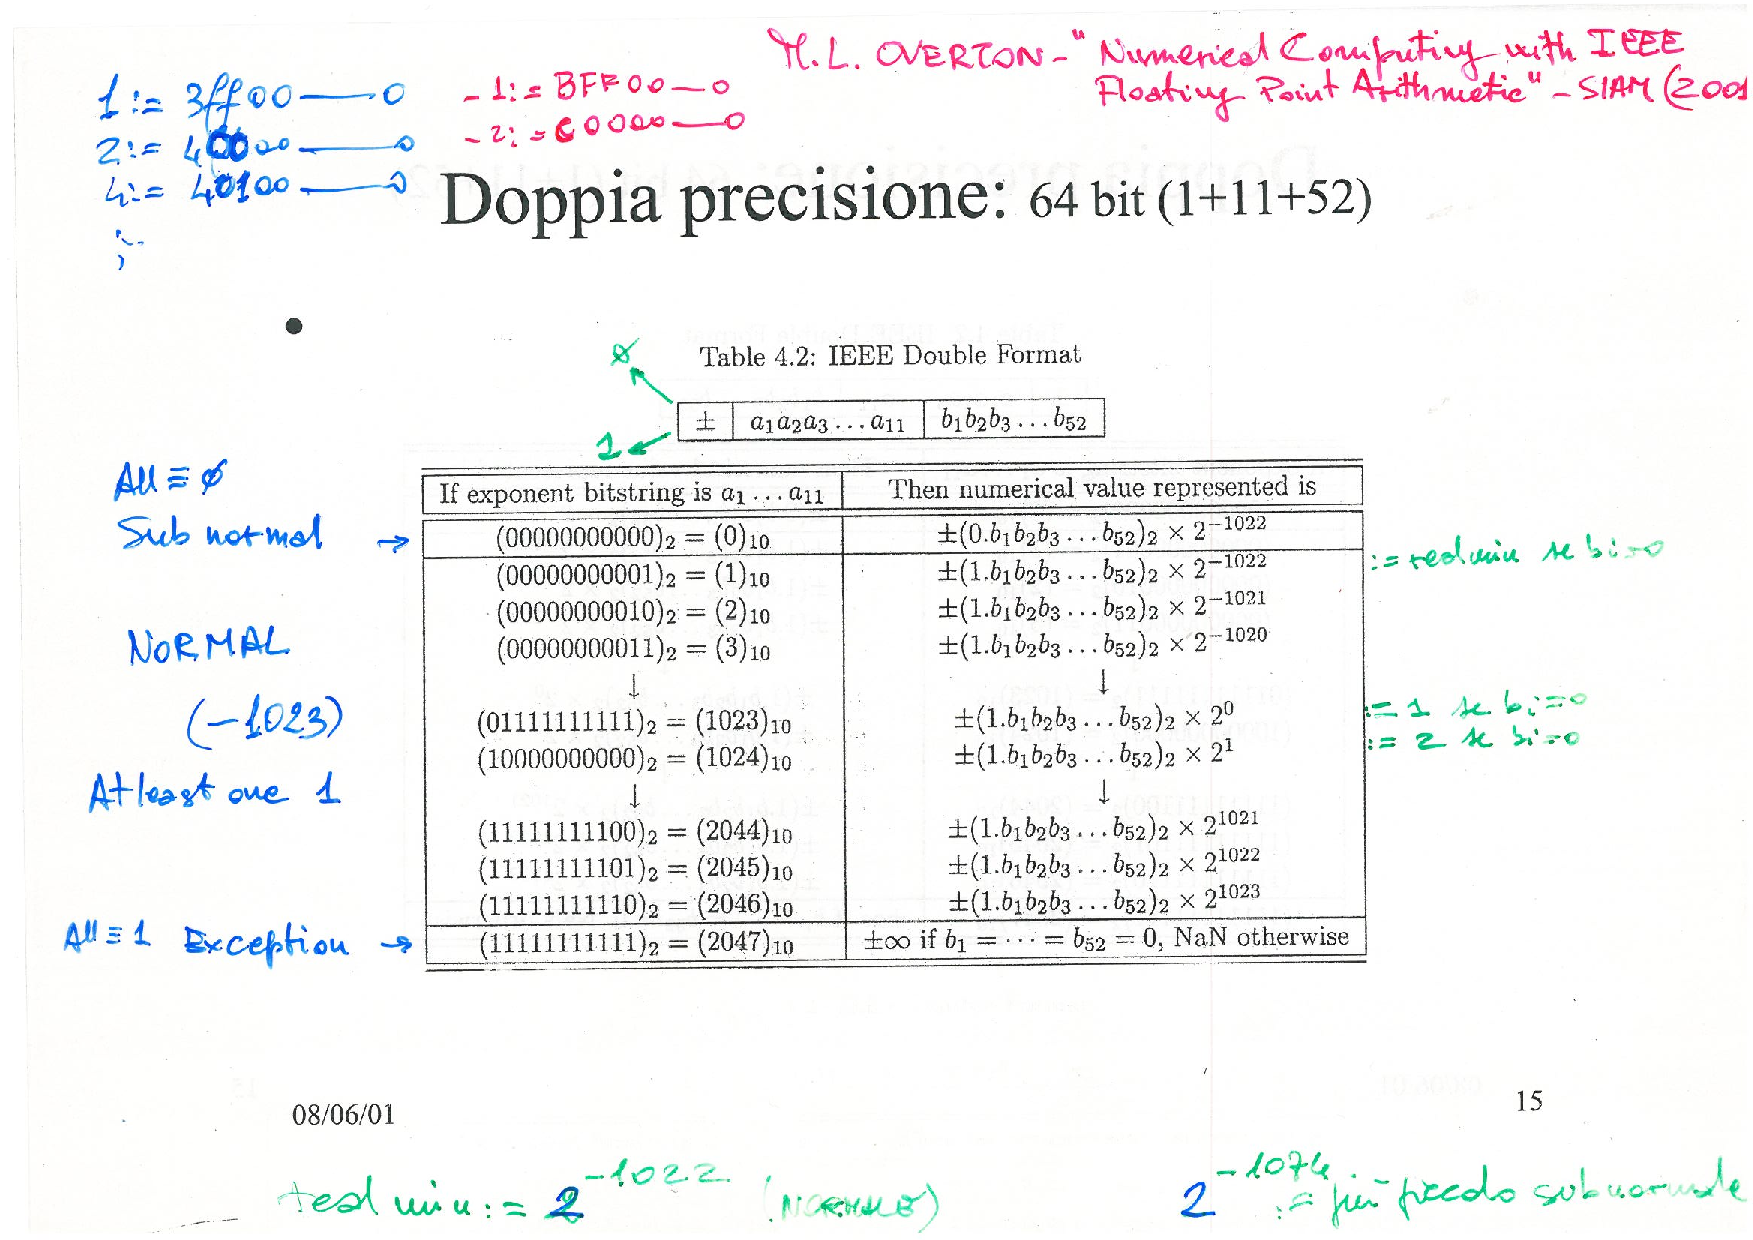
\includegraphics[width=.9\linewidth]{IEEE}
\end{frame}

\begin{frame}[fragile]
\frametitle{Excercise 1: IEEE double representation}

Write a {\tt C++} program that displays the byte 
representation of a double.

\end{frame}

\begin{frame}[fragile]
\frametitle{Excercise 1: IEEE double representation}

Write a {\tt C++} program that displays the byte 
representation of a double.

{\scriptsize
\begin{lstlisting}
#include <iostream>
#include <cstdint>

int main (void)
{

  union 
  {
    double d;
    unsigned char b[8];
  }  d;

  d.d = 2.0;
  for (int ii = 7; ii > 0; --ii)
    {      
      std::cout << static_cast<int> (d.b[ii]);
      std::cout << " ";
    }
  std::cout << std::endl;

  return 0;
}
\end{lstlisting}}
\end{frame}

\section{Shell scripting 101}

\begin{frame}[fragile]
\frametitle{Excercise 2: LaTeX slides build scripts}
Write an executable shell script that
\begin{enumerate}
\item Given the input argument {\tt "build"} builds these slides from the LaTeX sources
\item Given the input argument {\tt "clean"} removes all temporary files
\item Given the input argument {\tt "distclean"} removes all temporary files and the pdf file
\end{enumerate}
\end{frame}

\begin{frame}[fragile]
\frametitle{Excercise 2: LaTeX slides build scripts}
Write an executable shell script that
\begin{enumerate}
\item Given the input argument {\tt "build"} builds these slides from the LaTeX sources
{\tiny
\begin{lstlisting}[language=bash]
if [[ $1 = build ]]
then
    TEXINPUTS=../LATEX/: pdflatex $2
    TEXINPUTS=../LATEX/: pdflatex $2
    TEXINPUTS=../LATEX/: pdflatex $2
\end{lstlisting}}
\item Given the input argument {\tt "clean"} removes all temporary files
\item Given the input argument {\tt "distclean"} removes all temporary files and the pdf file
\end{enumerate}
\end{frame}

\begin{frame}[fragile]
\frametitle{Excercise 2: LaTeX slides build scripts}
Write an executable shell script that
\begin{enumerate}
\item Given the input argument {\tt "build"} builds these slides from the LaTeX sources
\item Given the input argument {\tt "clean"} removes all temporary files
{\tiny
\begin{lstlisting}[language=bash]
elif [[ $1 = clean ]]
then
    FILES=$(ls $2.*)   
    for file in ${FILES}
    do
        echo $file
        if [[ $file = $2.tex ]]
        then
            echo "do not delete $file"
        elif [[ $file = $2.pdf ]]
        then
            echo "do not delete $file"
        elif [[ $file != $2.tex ]] && [[ $file != $2.pdf ]]
        then
            rm $file
        fi        
    done
\end{lstlisting}
}
\item Given the input argument {\tt "distclean"} removes all temporary files and the pdf file
\end{enumerate}
\end{frame}

\begin{frame}[fragile]
\frametitle{Excercise 2: LaTeX slides build scripts}
Write an executable shell script that
\begin{enumerate}
\item Given the input argument {\tt "build"} builds these slides from the LaTeX sources
\item Given the input argument {\tt "clean"} removes all temporary files
\item Given the input argument {\tt "distclean"} removes all temporary files and the pdf file
{\tiny
\begin{lstlisting}[language=bash]
elif [[ $1 = distclean ]]
then
    FILES = $(ls $2.*)
    for file in ${FILES}
    do
        if [[ $file = $2.tex ]]
        then
            echo "do not delete $file"
        elif [[ $file != $2.tex ]]
        then
            rm $file
        fi        
    done
fi
\end{lstlisting}
}
\end{enumerate}
\end{frame}

\begin{frame}
\frametitle{More about {\tt bash}}

\begin{itemize}
\item {\tt bash} cheat-sheet attached
\item Advanced Bash Scripting Guide {\tt http://www.tldp.org/LDP/abs/html/abs-guide.html}
\end{itemize}

\end{frame}

\section{Makefile basics}
\frame{
\frametitle{Excercise 3: LaTeX slides make}
Write a Makefile that behaves like the script of Excercise 2
}

\frame{
\frametitle{Excercise 3: LaTeX slides make}
Write a Makefile that behaves like the script of Excercise 2\\
{\tiny
\lstinputlisting{./Makefile}
}}

\frame{
\frametitle{More on makefiles}
\begin{itemize}
\item More exercises on Makefiles in the folder {\tt 99-makefile}
\item GNU make documentation\\
{\tt http://www.gnu.org/software/make}
\end{itemize}
}

\section{Portability}
\frame{
\frametitle{Complex Makefiles for large projects}

There is one main thing you should know about Complex Makefiles for large projects:

\begin{center}
\emph \large \bf Don't write them!
\end{center}

For large complex projects you should use 
\begin{itemize}
\item Autotools
\begin{itemize}
\item {\tt http://www.gnu.org/software/automake}
\item {\tt http://www.gnu.org/software/autoconf}
\item {\tt http://www.gnu.org/software/libtool}
\end{itemize}

\item CMake
\begin{itemize}
\item {\tt http://www.cmake.org/}
\end{itemize}

\end{itemize}

To generate the makefiles.
}

\end{document}

